%  Last change by: Irina Tecker, 11-OCT-2016 
\chapter{Element Types}
\label{chap:elements}

\section{Marker}
\label{sec:marker}
\ttindex{marker}

\madbox{
label: MARKER;
}
The simplest element which can occur in a beam line is a
\texttt{MARKER}. It has zero length and has no effect on the beam, but
it allows one to identify a position in the beam line, for example to
apply a matching constraint.

\textbf{Example:}
\madxmp{M27: MARKER;}


\section{Drift Space}
\label{sec:drift}
\ttindex{drift}

\madbox{
label: DRIFT, L=real;
}

A drift space has one real attribute: 
\begin{madlist}
   \ttitem{L} The drift length (Default: 0 m) 
\end{madlist}

\textbf{Example:}
\madxmp{
DR1: \= DRIFT, \= L=1.5; \\
DR2: \> DRIFT, \> L=DR1->L;
}
The length of DR2 is always equal to the length of DR1.

The \hyperref[subsec:local-straight]{straight reference system} for a drift
space is a Cartesian coordinate system.   


\section{Bending Magnet}
\ttindex{bend}
\label{sec:bend}
Two different type keywords are recognised for bending magnets, they are
distinguished only by the reference system used:  
\begin{madlist}
  \ttitem{SBEND}\label{bend-sbend} is a sector bending magnet. \\
  The planes of the pole faces intersect at the centre of curvature of
  the curved \hyperref[subsec:local-rbend]{sbend reference system}.  
  \ttitem{RBEND}\label{bend-rbend} is a specific case of SBEND. \\ 
  The pole faces are parallel. The reference system is the curved  
  \hyperref[subsec:local-rbend]{rbend reference system}.
\end{madlist}

Bendig magnets are defined by the statements: 
\madbox{
label: SBEND, \= L=real, ANGLE=real, TILT=real, \\
              \> K0=real, K1=real, K2=real, KS=real,\\
              \> E1=real, E2=real, FINT=real, FINTX=real,\\ 
              \> HGAP=real, H1=real, H2=real,\\
              \> THICK=logical;\\
              \> \\
              \> \\
label: RBEND, \> L=real, ANGLE=real, TILT=real, \\
              \> K0=real, K1=real, K2=real, KS=real,\\
              \> E1=real, E2=real, FINT=real, FINTX=real, \\
              \> HGAP=real, H1=real, H2=real, \\
              \> THICK=logical, \\
              \> ADD\_ANGLE='array';
}

Bending magnets have the following attributes:
\begin{madlist}
   \ttitem{L} The length of the magnet (default: 0 m). \\
   For sector bends the declared length is the arc length 
   of the reference orbit. \\
   For rectangular bends the declared length is normally the length of a
   straight line joining the entry and exit points, as in the
   Figure. \\ 
   Internally \madx only uses the arc length of the reference orbit for
   both bend types.\\ 
   \textbf{In order to define \texttt{RBEND}'s with a declared length equal to the
     arc length of the reference orbit, the option \texttt{RBARC} must be
     previously set to FALSE in \madx with \texttt{Option, RBARC=false;}} 
   
   \ttitem{ANGLE} The bend angle (default: 0 rad). \\ 
   A positive bend angle represents a bend to the right, i.e. towards
   negative \textit{x} values.  
   
   \ttitem{ADD\_ANGLE} An array of (maximum 5) bending angles for
   multiple passes. See \texttt{ADD\_PASS} option of the
   \hyperref[chap:sequence]{\texttt{SEQUENCE}} command. This is only
   allowed for \texttt{RBEND} elements and is ignored for \texttt{SBEND}
   elements.
 
   \ttitem{TILT} The roll angle about the longitudinal axis (default: 0
   rad, i.e. a horizontal bend). \\ 
   A positive angle represents a clockwise rotation. \\ 
   An attribute \texttt{TILT=pi/2} turns a horizontal into a vertical
   bend, and a positive \texttt{ANGLE} then denotes a downwards
   deflection. 

   \ttitem{K1} The quadrupole coefficient (Default: 0 m$^{-2}$)\\
     $K_1 = (1/B\rho) (\partial B_y / \partial x)$. \\
   A positive quadrupole strength implies horizontal focussing of particles, 
   irrespective of their charge.
   % positively charged particles.  % Ghislain: sera chang� dans le futur! 

   \ttitem{E1} The rotation angle for the entrance pole face (Default: 0 rad). 
   \ttitem{E2} The rotation angle for the exit pole face (Default: 0 rad). \\
   The pole face rotation angles are referred to the magnet model for
   \hyperref[F-RBND]{rectangular bend} and \hyperref[F-SBND]{sector
     bend} respectively. \\ 
   \texttt{E1} and \texttt{E2} are positive if they reduce the length of the
   side of the bend that is further away from the centre of
   curvature. \\
   \texttt{E1} and \texttt{E2} must be specified as positive to give an
   \texttt{SBEND} parallel faces, i.e. turning it into an
   \texttt{RBEND}. \texttt{E1} and \texttt{E2} must be negative to give
   an \texttt{RBEND} faces whose planes intersect at the centrer of
   curvature, ie turning it into an \texttt{SBEND}.   

   \ttitem{FINT} The fringe field integral at entrance and exit of the
   bend. (Default:  0). 
   \ttitem{FINTX} If defined and positive, the fringe field integral at
   the exit of the element, overriding \texttt{FINT} for the
   exit. (Default: =\texttt{FINT}) \\  
   This allows to set different fringe field integrals at entrance
   (\texttt{FINT}) and exit (\texttt{FINTX}) of the element.  

   \ttitem{HGAP} The half gap of the magnet (default: 0 m). 

   \ttitem{K2} The sextupole coefficient. (Default: 0 m$^{-3}$) \\ 
   $K_2 = (1/B\rho) (\partial^2 B_y / \partial x^2)$.   

  \ttitem{KS} The skew quadrupole coefficient 
   $K_{s} = 1/(2 B \rho) (\partial B_x / \partial x - \partial B_y / \partial y)$\\  
    where (x,y) is a coordinate system rotated by $-45^\circ$ around s
    with respect to the normal one. The default is 0 m$^{-2}$. A
    positive skew quadrupole strength implies \textsl{defocussing}, 
    irrespective of the charge of the particles,  
    in the (x,s) plane rotated by $45^\circ$
    around \textit{s} (particles in this plane have \texttt{x = y $>$ 0}). 

   \ttitem{H1}The curvature of the entrance pole face. 
   (Default: 0 m$^{-1}$).   
   \ttitem{H2} The curvature of the exit pole face. (Default: 0 m$^{-1}$) \\
   A positive pole face curvature induces a negative sextupole
   component; i.e. for positive \texttt{H1} and \texttt{H2} the centres
   of curvature of the pole faces are placed inside the magnet. 

   \ttitem{K0} \textbf{OBSOLETE} \\
   Please take note that $K_0$ and $K_0s$ are left in the
   data base but are no longer used for the MAP of the bends,
   instead \texttt{ANGLE} and \texttt{TILT} are used exclusively. \\
   However, specifying \texttt{K0} is required in order to be able to
   assign \textbf{relative} field errors to a bending magnet because
   \texttt{K0} is used for the normalization instead of the
   \texttt{ANGLE}. (see \hyperref[sec:efcomp]{\texttt{EFCOMP}}).\\ 
   With $K_0 = (1 / B \rho) B_y$, one gets \texttt{K0 = ANGLE / arclength}.


   \ttitem{THICK} If this logical flag is set to true the bending 
   magnet is tracked through as a thick-element, instead of being
   converted into thin-lenses. \\
   (Default: false)

   \ttitem{KILL\_ENT\_FRINGE} If this logical flag is set to true the fringe fields on the entrance of the element are not taken into account (not calculated). \\
   (Default: false)

   \ttitem{KILL\_EXT\_FRINGE} If this logical flag is set to true the fringe fields on the exit of the element are not taken into account (not calculated). \\
   (Default: false)
\end{madlist}

\textbf{Note:} Additional attributes can be given to bending magnets; They
are useful for \ptc and are defined in \ref{sec:add-option-PTC}.

\vskip 5mm
\textbf{\underline{Fringe Fields:}}
\vskip 3mm
The quantities \texttt{FINT} and \texttt{HGAP} specify the finite extent
of the fringe fields as defined in SLAC-75 \cite{slac75}:
\begin{equation}
\mathrm{FINT}=\int_{-\infty}^\infty \frac{B_y(s)(B_0-B_y(s))}{g \cdot
  B_0^2}\,\mathrm{d}s ,\quad\quad g=2\cdot \mathrm{HGAP}. 
\end{equation}

The default values of zero corresponds to the hard-edge approximation,
i.e. a rectangular field distribution. For other approximations, enter
the correct value of the half gap, and one of the following values for
\texttt{FINT}: 
 
\begin{center}
  \begin{tabular}{l l}
    Linear Field drop-off                   &  1/6 \\
    Clamped "Rogowski" fringing field       &  0.4 \\
    Unclamped "Rogowski" fringing field     &  0.7 \\
    "Square-edged" non-saturating magnet    &  0.45
  \end{tabular}
\end{center}


Entering the keyword \texttt{FINT} alone sets the integral to 0.5, which is a
reasonable average of the above values.  

Note also that the possibility to specify both \texttt{FINT} and
\texttt{FINTX} allows one to set different values at entrance and exit
of a bend element. \\  
This can be particularly useful to set the fringe field integral to zero
on one side only, \textsl{e.g.} when slicing a dipole.  


\textbf{\underline {Examples:}}
\madxmp{
xxxxxxxxxxxxxxxxxxxxxxxxxxxxxxxxxxxxxxxxxxx\= \kill
BR: RBEND, L=5., ANGLE=+0.001;             \>! Deflection to the right \\
BD: RBEND, L=5., ANGLE=+0.001, TILT= pi/2; \>! Deflection down \\
BL: RBEND, L=5., ANGLE=+0.001, TILT= pi;   \>! Deflection to the left \\
BU: RBEND, L=5., ANGLE=+0.001, TILT=-pi/2; \>! Deflection up
}



\section{Dipole edge}
\ttindex{dipedge}
\label{sec:dipedge}

A thin element describing the edge focusing of a dipole has been
introduced in order to make it possible to track trajectories in the
presence of dipoles with pole face angles. Only linear terms are
considered since the higher order terms would make the tracking
non-symplectic. The transformation of the machine elements into thin
lenses leaves dipole edge (\texttt{DIPEDGE}) elements untouched and splits 
correctly the \texttt{SBEND}'s.  

It does not make sense to use a \texttt{DIPEDGE} alone. 
It can be specified at the entrance and the exit of a \texttt{SBEND}. 
A dipole edge element is defined by the command:  
\madbox{
  label: DIPEDGE, \= H=real, E1=real, FINT=real, \\
                  \> HGAP=real, TILT=real; 
}

A \texttt{DIPEDGE} has zero length and five attributes. 
\begin{madlist}
   \ttitem{H} Is angle/length or 1/rho (default: 0 m$^{-1}$ - for the
     default the dipedge element has no effect). (must be equal to that
     of the associated \texttt{SBEND})  
   \ttitem{E1} The rotation angle for the pole face. The sign convention is
     as for a \hyperref[bend-sbend]{\texttt{SBEND}} bending magnet. Note that it is
     different for an entrance and an exit. (default: 0 rad).  
   \ttitem{FINT} field integral as for \texttt{SBEND}
     \hyperref[F-SBND]{sector bend}. Note that each
     \texttt{DIPEDGE} has its own \texttt{FINT}, so that specifying
     \texttt{FINTX} is no longer necessary.   
   \ttitem{HGAP} half gap height of the associated \hyperref[bend-sbend]{\texttt{SBEND}}
     bending magnet.   
   \ttitem{TILT} The roll angle about the longitudinal axis (default: 0
     rad, \textsl{i.e.} a horizontal bend). A positive angle represents a
     clockwise rotation.  
\end{madlist}



%  Changed by: Andrea Latina, 6-May-2013 
\section{Quadrupole}
\ttindex{quadrupole}
\label{sec:quadrupole}

\madbox{
label: QUADRUPOLE, \= L=real, K1=real, K1S=real, TILT=real,\\
                   \> THICK=logical;
}


A \texttt{QUADRUPOLE} has five attributes:     
\begin{madlist}
   \ttitem{L} The quadrupole length (default: 0 m). 
   \ttitem{K1} The normal quadrupole coefficient:        
     $K_1 = 1/(B \rho) (\partial B_y / \partial x)$.\\ 
     The default is 0 m$^{-2}$. A positive normal quadrupole strength
     implies horizontal focussing, irrespective of the charge of the particles.
     % of positively charged particles.  
   \ttitem{K1S} The skew quadrupole coefficient 
     $K_{1s} = 1/(2 B \rho) (\partial B_x / \partial x - \partial B_y / \partial y)$\\  
     where (x,y) is now a coordinate system rotated by $-45^\circ$ around s
     with respect to the normal one. The default is 0 m$^{-2}$. A
     positive skew quadrupole strength implies \textsl{defocussing}, 
     irrespective of the charge of the particles,  
     % of positively charged particles 
     in the (x,s) plane rotated by $45^\circ$
     around \textit{s} (particles in this plane have \texttt{x = y $>$ 0}). 
   \ttitem{TILT} The roll angle about the longitudinal axis (default: 0
     rad, i.e. a normal quadrupole). A positive angle represents a
     clockwise rotation. A \texttt{TILT=pi/4} turns a positive normal quadrupole
     into a negative skew quadrupole.          

   \textbf{Please note that contrary to \madeight one has to
     specify the desired TILT angle, otherwise it is taken as
     0 rad. This was needed to avoid the confusion in \madeight
     about the actual meaning of the \texttt{TILT} attribute for
     various elements.} 

    \ttitem{THICK} If this logical flag is set to true the quadrupole
    is tracked through as a thick-element, instead of being
    converted into thin-lenses.\\
    (Default: false)
\end{madlist}

\textbf{Note also that $K_1$ or $K_{1s}$ can be considered as
  the normal or skew quadrupole components of the magnet on
  the bench, while the TILT attribute can be considered as a
  tilt alignment error in the machine. In fact, a positive
  $K_1$ with a \texttt{TILT = 0} is equivalent to a positive $K_{1s}$
  with \texttt{TILT = +$\pi/4$ }} 

Example: 
\madxmp{QF: QUADRUPOLE, L=1.5, K1=0.001, THICK=true;}

%irina 
\textbf{Note:} Quadrupoles doesn't carry any attributes of bending magnet or sextupole, i.e. $K_0$ or $K_2$. In case these have to be considered in the element, please use multipole or bending magnet as a type of an element.


\textbf{Note:} Additional attributes can be given to quadrupoles; They
are useful for \ptc and are defined in \ref{sec:add-option-PTC}.

The \hyperref[subsec:local-straight]{straight reference system} for
a quadrupole is a Cartesian coordinate system.


\section{Sextupole}
\ttindex{sextupole}
\label{sec:sextupole}

\madbox{
label: SEXTUPOLE, L=real, K2=real, K2S=real, TILT=real;
}

A \texttt{SEXTUPOLE} has four real attributes: 
\begin{madlist}
    \ttitem{L} The sextupole length (default: 0 m). 
    \ttitem{K2} The normal sextupole coefficient $K_2 = \frac{1}{B \rho}
      (\partial^2 B_y / \partial x^2)$. \\       
      (default: 0 m$^{-3}$). 
    \ttitem{K2S} The skew sextupole coefficient 
      $K_{2S} = \frac{1}{B \rho} (\partial^2 B_x / \partial x^2)$ \\
%% 2013-Jul-05  17:58:30  ghislain: error reported by Christian Carli
%      \textit{K}$_{2S}$ = 1/(2 \textit{B} rho)
%      ($\partial$$^2$\textit{B$_x$}/$\partial$ \textit{x}$^2$ -
%      $\partial$$^2$\textit{B$_y$}/$\partial$ \textit{y}$^2$).   
      where (x,y) is now a coordinate system rotated by $-30^\circ$ around s with
      respect to the normal one. (default: 0 m$^{-3}$). A positive skew
      sextupole strength implies \textsl{defocussing} (!) 
      irrespective of the charge of the particles,
      % of positively charged particles 
      in the (x,s) plane rotated by $30^\circ$ around s (particles in
      this plane have $x > 0$, $y > 0$).  

    \ttitem{TILT} The roll angle about the longitudinal axis (default: 0
      rad, i.e. a normal sextupole). A positive angle represents a
      clockwise rotation. A \texttt{TILT = pi/6} turns a positive normal 
      sextupole into a negative skew sextupole.
      
      \textbf{Please note that contrary to \madeight one has to specify the
        desired \texttt{TILT} angle, otherwise it is taken as
        0~rad. This was needed to avoid the confusion in \madeight about
        the actual meaning of the \texttt{TILT} attribute for various
        elements.}  
\end{madlist}

\textbf{Note also that $K_2$ or $K_{2s}$ can be considered as the normal
  or skew sextupole components of the magnet on the bench, while the
  \texttt{TILT} attribute can be considered as an tilt alignment error in the
  machine. In fact, a positive $K_2$ with a $\mathtt{TILT} = 0$ is equivalent to a
  positive $K_{2s}$ with positive $\mathtt{TILT} = \pi/6$.} 

Example: 
\madxmp{S: SEXTUPOLE, L=0.4, K2=0.00134;}

%irina 
\textbf{Note:} Sextupole doesn't carry any attributes of bending magnet or quadrupole,
 i.e. $K_0$ or $K_1$t. In case these have to be considered in the element, please use 
 multipole or bending magnet as a type of an element.


\textbf{Note:} Additional attributes can be given to sextupoles; They
are useful for \ptc and are defined in \ref{sec:add-option-PTC}.

The \hyperref[subsec:local-straight]{straight reference system} for a
sextupole is a Cartesian coordinate system.   


\section{Octupole}
\ttindex{octupole}
\label{sec:octupole}

\madbox{
label: OCTUPOLE, L=real, K3=real, K3S=real, TILT=real;
}

An \texttt{OCTUPOLE} has four real attributes: 
\begin{madlist}
   \ttitem{L} The octupole length (default: 0 m). 

   \ttitem{K3} The normal octupole coefficient 
     $K_3 = \frac{1}{B \rho} (\partial^3B_y / \partial x^3)$ \\ 
     (default:  0 m$^{-4}$). 

   \ttitem{K3S} The skew octupole coefficient 
%% 2013-Jul-05  18:00:59  ghislain: to be checked wrt error reported on
%% K2S for sextupoles 
     $K_{3S} = \frac{1}{2 B\rho} (\partial^3B_x/\partial x^3 -
   \partial^3B_y/\partial y^3)$ \\
     where (x,y) is now a coordinate system rotated by -22.5$^o$ around
     s with respect to the normal one. (default: 0 m$^{-4}$). A positive
     skew octupole strength implies \textsl{defocussing} (!) 
     irrespective of the charge of the particles,
     % of positively charged particles 
     in the (x,s) plane rotated by 22.5$^o$ around s
     (particles in this plane have x $>$ 0, y $>$ 0).  

   \ttitem{TILT} The roll angle about the longitudinal axis (default: 0
     rad, i.e. a normal octupole). A positive angle represents a
     clockwise rotation. A \texttt{TILT=pi/8} turns a positive normal octupole
     into a negative skew octupole.  

     \textbf{Please note that contrary to \madeight one has to specify the
       desired TILT angle, otherwise it is taken as 0 rad. This was
       needed to avoid the confusion in \madeight about the actual meaning of
       the TILT attribute for various elements. }

\end{madlist}

\textbf{Note also that $K_3$ or $K_{3S}$ can be considered as the normal or
  skew quadrupole components of the magnet on the bench, while the
  \texttt{TILT} attribute can be considered as an tilt alignment error
  in the machine. In fact, a positive $K_3$ with a \texttt{TILT=0} is
  equivalent to a positive $K_{3S}$ with positive \texttt{TILT=+pi/8}.} 

Example: 
\madxmp{O3: OCTUPOLE, L=0.3, K3=0.543;}

\textbf{Note:} Additional attributes can be given to octupoles; They
are useful for \ptc and are defined in \ref{sec:add-option-PTC}.

The \hyperref[subsec:local-straight]{straight reference system} for a
octupole is a Cartesian coordinate system. Octupoles are normally
treated as thin lenses, except when tracking by Lie-algebraic methods.   



\section{General Thin Multipole}
\ttindex{multipole}
\label{sec:multipole}

A \texttt{MULTIPOLE} is a thin-lens magnet of arbitrary order, including a 
dipole component.

\madbox{
label: MULTIPOLE, \= LRAD=real, TILT=real, \\
                  \> KNL=\{real, \ldots \}, KSL=\{real, \ldots \};
}

\begin{madlist}
    \ttitem{LRAD} A fictitious length, originally only used to
      compute synchrotron radiation effects. \\
      A non-zero \texttt{LRAD} in conjunction with
      \hyperref[sec:option]{\texttt{OPTION, THIN\_FOC=true}}
      takes into account the weak focussing of bending magnets.
      
    \ttitem{TILT} The roll angle about the longitudinal axis (default: 0
      rad). A positive angle represents a clockwise rotation of the
      multipole element. The roll angle affects all components.
      
    \ttitem{KNL} An array of the integrated normal multipole coefficients, 
      starting from order zero and up to the maximum order (currently 20). 
      The parameters are positional in the array, therefore 
      zeros must be filled in for components that do not exist. \\
      The coefficient of rank $i$ in the array corresponds to the integrated 
      strength $K_i L = B_i . L / (B\rho)$ where the strength is given by 
      equation \ref{eq:kn}. 
      Hence the first argument of the array, the argument for a normal
      multipole of order zero, $K_0 L = B_0 . L / (B\rho)$ is equal to
      the normal horizontal rotation angle of the thin dipole.
      
    \ttitem{KSL} An array of the integrated skew multipole coefficients, 
     starting from order zero and up to the maximum order (currently 20). The
     parameters are positional in the array, therefore zeros must be
     filled in for components that do not exist. 
     Hence the first argument of the array, the argument for a skew
     multipole of order zero, $K_0 L = B_0 . L / (B\rho)$ is equal to
     the skew or vertical rotation angle of the thin dipole.
 
\end{madlist}

Both \texttt{KNL} and \texttt{KSL} may be specified for the same multipole. 

Contrary to \madeight the desired \texttt{TILT} angle must be explicitly
specified, and defaults otherwise to 0 rad. The roll angle specified
with \texttt{TILT} is global to all multipolar components.  
Hence the \texttt{KNL} and \texttt{KSL} components can be considered as the
normal or skew multipole components of the magnet as measured on the
bench, while the \texttt{TILT} attribute can be considered as an alignment
error as measured in the machine.

A multipole with no dipole component has no effect on the reference
orbit, i.e. the reference system at its exit is the same as at its
entrance. If it includes a dipole component, it has the same effect on
the reference orbit as a dipole with zero length, total deflection 
\texttt{angle} and \texttt{tilt} defined by:
\begin{equation}
  \begin{aligned}
    \mathtt{angle} &= \sqrt{ \mathtt{KNL}(0)^2 + \mathtt{KSL}(0)^2 }\\
    \mathtt{tilt}  &= \arctan (\mathtt{KSL}(0) / \mathtt{KNL}(0))  
  \end{aligned}
\end{equation}
Note that the global \texttt{TILT} attribute of the \texttt{MULTIPOLE}
is then added to the intrinsic \texttt{tilt} calculated from
\texttt{KNL} and \texttt{KSL}. 

%In order to know the current maximum order of a given multipole, use the
%command \texttt{HELP, MULTIPOLE;} and count.


\textbf{Examples:}\\
A thin-lens sextupole:  
\madxmp{ms: MULTIPOLE, KNL=\{0, 0, k2l\};}

A thin-lens skew octupole:  
\madxmp{mso: MULTIPOLE, KSL=\{0, 0, 0, k3sl\};}

A thin-lens multipole with a normal octupole component and a skew decapole
component:
\madxmp{mod: MULTIPOLE, KNL=\{0,0,0,myoct*lrad\}, KSL=\{0,0,0,0,-1.e-5\};}

A thin-lens dipole bending to the right and down for a total angle of
2 milliradians and a tilt of $\pi/4$ can be equivalently defined as:
\madxmp{
hvbend: MULTIPOLE, KNL=\{1.414e-3\}, KSL=\{1.414e-3\};\\
hvbend: MULTIPOLE, KNL=\{2.e-3\}, TILT= pi/4;\\
hvbend: MULTIPOLE, KSL=\{2.e-3\}, TILT=-pi/4;
}



% moved from element format above
% commented by Ghislain on 2014-01-01
%A special format is used for a \href{multipole.html}{multipole}\index{multipole}: 
%\madxmp{
%m: multipole, \= knl= \{kn0, kn1, kn2, ..., knmax\}, \\
%              \> ksl= \{ks0, ks1, ks2, ..., ksmax\};
%}
%where knl and ksl give the integrated normal and skew strengths,
%respectively. The commas are mandatory, each strength can be an
%expression; their position defines the order.



%  Changed by: Alexander Koschik, 16-May-2006 
\section{Solenoid}
\ttindex{solenoid}
\label{sec:solenoid}

Solenoids can be defined in two forms, a thick and a thin version: 

\madbox{
xxxxxxxxxxxxxxxxxxxxxxxxxx\=xxxxxxxxxxxxxxxxxxx\= \kill
label: SOLENOID, L=real,  \>KS=real;           \> ! thick version \\ 
label: SOLENOID, L=0,     \>KS=real, KSI=real; \> ! thin version 
}

A \texttt{SOLENOID} has three real attributes: 
\begin{madlist}
   \ttitem{L} The length of the solenoid (default: 0 m) 
   \ttitem{KS} The solenoid strength $K_s = B_0 / B\rho$ (default: 0
     rad/m). For positive \texttt{KS} and positive particle charge, the
     solenoid field points in the direction of increasing $s$.  
   \ttitem{KSI} The solenoid integrated strength $K_s L$
     (default: 0 rad).  This additional attribute is needed only when
     using the thin solenoid,  where $L=0$.     
\end{madlist}

Example: 
\madxmp{
xxxxxxxxxx\=xxxxxxxxxxxxxxxxxxxx\= \kill
SOLO:     \> SOLENOID, L = 2., \> KS = 0.001; \\
THINSOLO: \> SOLENOID, L = 0,  \> KS = 0.001, KSI = 0.002;
}

\textbf{Note:} Additional attributes can be given to solenoids. They
are useful for \ptc and are defined in \ref{sec:add-option-PTC}.
In particular multipole coefficients \texttt{KNL} and \texttt{KSL} can
also be specified for solenoids. They have no effect in \madx proper but
are used in \ptc for solenoid with multipoles.

The \hyperref[subsec:local-straight]{straight reference system} for a
solenoid is a Cartesian coordinate system. 
 


\section{Nonlinear Lens with Elliptic Potential}
\ttindex{nllens}
\label{sec:nllens}

\madbox{
label: NLLENS, KNLL=real, CNLL=real;
}

The \texttt{NLLENS} element represents a thin nonlinear lens with the potential
of 'Elliptic' type as specified in \cite{danilov2010}. The lens is used
to create fully integrable 2D nonlinear accelerator lattice with very
large nonlinear tune spread/shift. The \texttt{NLLENS} element is recognized by
the thin tracking module. The quadrupole term of the potential is
included in the transport map and, consequently, affects the calculation
of tunes and Twiss functions.   

\begin{madlist}
   \ttitem{KNLL} The integrated strength of lens (m). The strength is
     parametrized so that the quadrupole term of the multipole
     expansion is \texttt{k1=2*KNLL/CNLL\textasciicircum2}.      
   \ttitem{CNLL} The dimensional parameter of lens (m). The singularities
     of the potential are located at X=-CNLL,+CNLL and Y=0.  
\end{madlist}

The scalar potential function of the element is given by
\begin{equation}
U(x,y)=\frac{k}{c}\frac{\xi\sqrt{\xi^2-1} \, \text{acosh}\xi +  
  \eta\sqrt{1-\eta^2}(\text{acos}\eta-\pi/2)}{\xi^2-\eta^2}
\end{equation}
\\ where \textit{k} = KNLL, \textit{c} = CNLL and 
\begin{equation}
\xi = \frac{\sqrt{(x+c)^2+y^2}+\sqrt{(x-c)^2+y^2}}{2c}, 
\quad \eta = \frac{\sqrt{(x+c)^2+y^2}-\sqrt{(x-c)^2+y^2}}{2c},
\end{equation}

Figure below shows the contour plot of the scalar potential: \\
\begin{figure}
  \centering
  %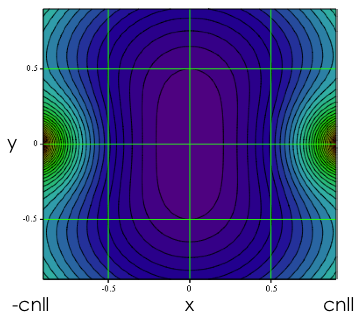
\includegraphics[width=220bp]{png/nllens_potential-2D.png}
  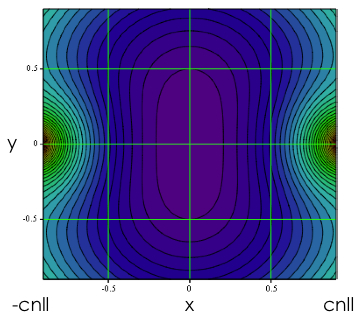
\includegraphics[width=220bp]{jpg/nllens_potential-2D.jpg}
  \caption{Contour plot of the scalar potential}
  \label{fig:nllens-potential}
\end{figure}

The multipole expansion of the scalar potential is \\
\begin{equation}
U(x,y)=k\cdot Re\left\{ \left(\dfrac{x + i y}{c}\right)^2 + 
\frac{2}{3}\left(\dfrac{x + i y}{c}\right)^4 +
\frac{8}{15}\left(\dfrac{x + i y}{c}\right)^6 + 
\frac{16}{35}\left(\dfrac{x + i y}{c}\right)^8 + \cdots \right\}
\end{equation}
\\ 
Note that this expansion is only valid inside the \textit{r=c} circle on
the x,y plane.    

In order to create integrable optics, one needs to shape the potential
along z axis according to the beta-function. Below is an example
nonlinear section representing the necessary nonlinear field with 20
thin lenses:  
\begin{verbatim}
    mu0 = 0.3;  ! phase advance over straight section
    l0 = 2.0;   ! length of the straight section
    nn = 20;    ! number of nonlinear elements
    tn = 0.45;  ! strength of nonlinear lens
    cn = 0.01;  ! dimentional parameter of nonlinear lens

    musect = mu0 + 0.5;
    f0 = l0/4.0*(1.0+1.0/tan(pi*mu0)^2);
    betae = l0/sqrt(1.0-(1.0-l0/2.0/f0)^2);
    alfae = l0/2.0/f0/sqrt(1.0-(1.0-l0/2.0/f0)^2);
    betas = l0*(1-l0/4.0/f0)/sqrt(1.0-(1.0-l0/2.0/f0)^2);
    value, f0, betae, alfae, betas;

    ncreate(ii,kk,cc): macro = {n.ii: nllens, knll=kk, cnll=cc;};

    i=0;
    while(i <  nn)
      {
        i = i+1;
        sn = l0/nn*(i-0.5);
        bn = l0*(1-sn*(l0-sn)/l0/f0)/sqrt(1.0-(1.0-l0/2.0/f0)^2);
        knn = l0*tn*cn^2/nn/bn;
        cnn = cn*sqrt(bn);
        exec, ncreate($i,knn,cnn);
        value, i, bn, cnn, knn;
      };
\end{verbatim}


%% To be moved in References at the end of the document
%% References:
%% \begin{enumerate}
%% \item V. Danilov, S. Nagaitsev, Phys. Rev. ST Accel. Beams \textbf{13},
%%   084002 (2010). 
  
%% \item A. Valishev, S. Nagaitsev, V. Kashikhin, V. Danilov, in
%%   Proceedings of 2011 Particle Accelerator Conference, New York, NY,
%%   USA, WEP070. 
%% \end{enumerate}

%A. Valishev, March 19, 2012


%  Changed by: Frank Schmidt, 28-Aug-2003 
%  Changed by: Werner Herr, 22-May-2007 
\section{Closed Orbit Corrector}
\ttindex{kicker}\index{orbit corrector}
\label{sec:closed-orbit-cor}\label{sec:kicker}

Three types of magnetic closed orbit correctors are available: 
\begin{madlist}
   \ttitem{HKICKER} a corrector for the horizontal plane, 
   \ttitem{VKICKER} a corrector for the vertical plane, 
   \ttitem{KICKER} a corrector for both planes. 
\end{madlist}

\madbox{
xxxxxxxxxxxxxxxx\=xxxxxxxxxxxxxxxxxxxx\= \kill
label: HKICKER, \>L=real, KICK=real,  \>TILT=real; \\
label: VKICKER, \>L=real, KICK=real,  \>TILT=real; \\
label: KICKER,  \>L=real, HKICK=real, \>VKICK=real, TILT=real;
}

\textbf{The type \texttt{KICKER} should not be used when an orbit corrector
  kicks only in one plane.}

The attributes have the following meaning: 
\begin{madlist}
   \ttitem{L} The length of the closed orbit corrector (default: 0 m). 
   \ttitem{KICK} The momentum change $\delta PX = \delta p_x/p_0$ or 
     $\delta PY = \delta p_y / p_0$ for respectively horizontal or vertical
     correctors. (default: 0).  
   \ttitem{HKICK} The horizontal momentum change 
     $\delta PX = \delta p_x/p_0$ for a corrector acting in both planes
     (default: 0).  
   \ttitem{VKICK} The vertical momentum change 
     $\delta PY = \delta p_y/p_0$  for a corrector acting in both planes
     (default: 0).  
   \ttitem{TILT} The roll angle about the longitudinal axis (default: 0
     rad). A positive angle represents a clockwise rotation of the
     kicker.  
\end{madlist}

A positive kick increases $p_x$ or $p_y$ respectively. This
means that a positive horizontal kick bends to the left,  i.e. to
positive $x$ which is opposite of what is true for bends.    

The deviation angle $\theta$ of the particle trajectory is related to
the momentum change through  $\sin \theta = \delta P = \delta p / p_0$.

It should be noted that the kick values assigned to an orbit corrector
like above are not overwritten by an orbit correction using the 
\hyperref[sec:correct]{\texttt{CORRECT}}
command. Instead the kicks computed by an orbit correction and the
assigned values are added when the correctors are used.  

 Examples: 
\madxmp{
xxxxxxx\=xxxxxxxxxx\=xxxxxxxxxxxxxxxxx\= \kill
HK1:   \>HKICKER, \>KICK = 0.001;  \\
VK3:   \>VKICKER, \>KICK = 0.0005; \\
VK4:   \>VKICKER, \>KICK := AVK4; \\
KHV1:  \>KICKER,  \>HKICK = 0.001,   \>VKICK = 0.0005; \\
KHV2:  \>KICKER,  \>HKICK := AKHV2H, \>VKICK := AKHV2V;
}

The assignment in the form of a deferred expression has the advantage
that the values can be assigned and/or modified at any time (and
matched!).   

The \hyperref[subsec:local-straight]{straight reference system} for an
orbit corrector is a Cartesian coordinate system.  


Please note that there is a new feature introduced by Stefan Sorge from
GSI. Here his decription:

The elements \texttt{KICKER, HKICKER}, and \texttt{VKICKER} can also be used as 
magnetic exciters providing sinusoidal momentum kicks. The usage in this case 
is:

\madxmp{
xykick: KICKER,  \= SINKICK=integer, SINPEAK=real, SINTUNE=real, SINPHASE=real;  \\
xkick : HKICKER, \> SINKICK=integer, SINPEAK=real, SINTUNE=real, SINPHASE=real;  \\
ykick : VKICKER, \> SINKICK=integer, SINPEAK=real, SINTUNE=real, SINPHASE=real;  
}
where a sinusoidal momentum kick \texttt{dpz} as a function of the  revolution
number \texttt{n} given by\\   
\texttt{dpz(n)=SINPEAK * sin(2*PI*SINTUNE*n + SINPHASE), pz=px,py} \\ 
is provided. 

The \texttt{KICKER} element generates synchronous kicks in both horizontal and
vertical planes. \texttt{HKICKER} generates only a horizontal kick, and
\texttt{VKICKER} generates only a vertical kick.    

The variables are 

\begin{madlist}
   \ttitem{SINKICK} must be set to 1 to switch on the sinusoidal
     signal, default: 0.  
   \ttitem{SINPEAK} amplitude of the bending angle (rad); default: 0
     rad.   
   \ttitem{SINTUNE} frequency of the signal times the revolution
     frequency.  Hence, the phase per revolution is 2*PI*SINTUNE;
     default: 0.   
   \ttitem{SINPHASE} initial phase; default: 0 rad.  
\end{madlist}

The momentum kick of a kicker has only a single frequency. An element
having a finite bandwidth can approximately created by defining  thin
kickers with all amplitudes \texttt{SINPEAK}, frequencies
\texttt{SINTUNE}, and initial phases \texttt{SINPHASE} desired and
putting them at the same position \textit{s} in the accelerator.

%From S.Sorge@gsi.de  


%  Created by: Laurent Deniau, 15-Sep-2011 
\section{Transverse Kicker}
\ttindex{tkicker}
\label{sec:tkicker}

The type \texttt{TKICKER} should be used to create horizontal, vertical or
combined transverse magnetic kickers physically equivalent to elements of type
\texttt{KICKER}, but \textbf{not used} by the \hyperref[sec:correct]{CORRECT} 
command of the closed orbit correction module.

Examples of elements that may use the type \texttt{TKICKER}: 
\begin{itemize}
   \item Fast kickers for injection, dump and tune
   \item Magnetic septa towards beam dump
   \item Dampers of transverse beam oscillations
   \item Undulator and Wiggler magnets
\end{itemize}

For further information on element type \texttt{TKICKER} and its attributes, look
at the documentation of the orbit corrector type
\hyperref[sec:kicker]{\texttt{KICKER}}.   

\section{RF Cavity}
\ttindex{RFcavity}
\label{sec:rf-cavity}\label{sec:rfcavity}

\madbox{
label: RFCAVITY, \= L=real, VOLT=real, LAG=real, \\
                 \> FREQ=real, HARMON=integer, \\    
                 \> N\_BESSEL=integer, NO\_CAVITY\_TOTALPATH=logical;
}

An \texttt{RFCAVITY} has eight real attributes and one integer attribute: 
\begin{madlist}
   \ttitem{L} The length of the cavity (DEFAULT: 0 m) 

   \ttitem{VOLT} The peak electrical RF voltage (DEFAULT: 0 MV). The effect of 
   the cavity is \\
     delta(\textit{E}) = VOLT * sin(2$\pi$ * (LAG - HARMON * \textit{f$_0$ t})). 

   \ttitem{LAG} The phase lag [$2\pi$] (DEFAULT: 0). 

   \ttitem{FREQ} The frequency [MHz] (no DEFAULT).  \\[3mm]
   \textbf{Note that if the RF frequency is not given, it is computed
     from the harmonic number and the revolution frequency
     \textit{f$_0$}. For accelerating structures this makes no sense,
     and the input of the frequency is mandatory.}   

   \ttitem{HARMON} The harmonic number \textit{h} (no DEFAULT). This
   attribute is only used if the frequency is not given.  
\end{madlist}

\textbf{Caveats:}
\begin{itemize}
  \item Please take note, that the following \madeight attributes:
    \texttt{BETRF, PG, SHUNT} and \texttt{TFILL} are currently not implemented in 
    \madx.    
%  \item BETRF: RF coupling factor (DEFAULT: 0).
%  \item PG: The RF power per cavity (DEFAULT: 0 MW).
%  \item SHUNT: The relative shunt impedance (DEFAULT: 0 MOhm/m).
%  \item TFILL: The filling time of the cavity $T_{fill}$ (DEFAULT: 0 microseconds). 

  \item Important Note: The \hyperref[chap:twiss]{\texttt{TWISS}} command
    is 4D only. As a consequence the \texttt{TWISS} parameters in the plane
    of non-zero dispersion may not close as expected. Therefore, it is best
    to perform \texttt{TWISS} in 4D only, \textsl{i.e.} with cavities
    switched off. If 6D is needed one has to use the
    \hyperref[sec:ptc-twiss]{\texttt{PTC\_TWISS}} command.  
\end{itemize}

The \texttt{RFCAVITY} can also have attributes that only become active in 
\ptc: 
\begin{madlist}
   \ttitem{N\_BESSEL} (DEFAULT: 0): \\
     Transverse focussing effects are typically ignored in the cavity in
     \madx or even \ptc. This effect is being calculated to order
     \texttt{n\_bessel}, with \texttt{n\_bessel=0} disregarding this
     effect and with a correct treatment when \texttt{n\_bessel} goes to
     infinity. 
   \ttitem{NO\_CAVITY\_TOTALPATH} (Default: false): \\
     flag to select whether the transit time factor in the cavity is to be
     considered (\texttt{NO\_CAVITY\_TOTALPATH = false}) or if the particle is
     kept on the crest of RF voltage (\texttt{NO\_CAVITY\_TOTALPATH = true}).  
\end{madlist}

A cavity requires the particle \hyperref[sec:beam]{\texttt{ENERGY}}
and the particle \hyperref[sec:beam]{\texttt{CHARGE}} to be set by a
\hyperref[sec:beam]{\texttt{BEAM}} command before any calculations are
performed. 

Example: 
\madxmp{
BEAM, PARTICLE=ELECTRON, ENERGY=50.0; \\
CAVITY: RFCAVITY, L=10.0, VOLT=150.0, LAG=0.0, HARMON=31320;
}

The \hyperref[subsec:local-straight]{straight reference system} for a
cavity is a Cartesian coordinate system.  


\section{Thin Radio-Frequency Multipole}
\ttindex{rfmultipole}
\label{sec:rfmultipole}

\madbox{
xxxxxxxxxxxxxxxxxxxxx\= \kill
label: RFMULTIPOLE, \>L=real, VOLT=real, LAG=real, \\
       \> FREQ=real, HARMON=integer, \\
       \> LRAD=real, TILT=real, \\
       \> KNL=\{real, \ldots \}, KSL=\{real, \ldots \}, \\
       \> PNL=\{real, \ldots \}, PSL=\{real, \ldots \};
}

A \texttt{RFMULTIPOLE} is a element which exhibits the properties
of an RF cavity as well as those of a multipole, of arbitrary order, oscillating at
the same RF frequency.

The accelerating kick is \texttt{delta(E) = VOLT * sin(2$\pi$ * (LAG - HARMON *
f0 t))}, and the multipole moments oscillate with the same RF frequency.
 
An \texttt{RFMULTIPOLE} requires the particle
\hyperref[sec:beam]{\texttt{ENERGY}} and the particle 
\hyperref[sec:beam]{\texttt{CHARGE}} to be set with a
\hyperref[sec:beam]{\texttt{BEAM}} command before any calculation is
performed.  

Contrary to the regular multipole, where the dipole
component has no effect on the reference orbit, an RF-Multipole that
includes a dipole component bends also the reference orbit.      
 
\begin{madlist}
   \ttitem{VOLT} The peak voltage of the RF accelerating mode (DEFAULT: 0 MV).
   \ttitem{LAG} The phase lag [$2\pi$] (DEFAULT: 0) 
   \ttitem{FREQ} The frequency [MHz] (no DEFAULT). \\ 
     Note that if the RF
     frequency is not given, it is computed from the harmonic
     number and the revolution frequency f0 as before. However, for
     accelerating structures this makes no sense, and the frequency
     is mandatory.  
   \ttitem{HARMON} The harmonic number h (no DEFAULT). Only if the
     frequency is not given. 
   \ttitem{LRAD} A fictitious length, which was originally just used to
     compute synchrotron radiation effects. A non-zero \texttt{LRAD} in
     conjunction with \hyperref[sec:option]{\texttt{OPTION, thin\_foc =
     true;}} takes into account the weak focussing of bending magnets.  
   \ttitem{TILT} The roll angle about the longitudinal axis (default: 0
     rad). A positive angle represents a clockwise rotation of the
     multipole element.            

     \textbf{Please note that contrary to \madeight one has to specify the
       desired \texttt{TILT} angle, otherwise it is taken as 0 rad. We
       believe that the \madeight concept of having individual
       \texttt{TILT} values for each component and on top with default
       values led to considerable confusion and allowed for excessive
       and unphysical freedom. Instead, in \madx the \texttt{KNL, KSL}
       components can be considered as the normal or skew
       multipole components of the magnet on the bench, while the
       \texttt{TILT} attribute can be considered as an tilt alignment
       error in the machine.} 

   \ttitem{KNL} An array of the integrated normal rfmultipole
     coefficients, starting from order zero and up to the maximum
     order (currently 20). 
     The parameters are positional in the array, therefore leading 
     zeros must be filled in for components that do not exist. 
%     The normal rfmultipole coefficients from order zero to
%     the maximum; the parameters are positional, therefore zeros
%     must be filled in for components that do not exist. Example of
%     a thin-lens sextupole: ms:rfmultipole, knl:=\{0, 0, k2l\}; 
   \ttitem{KSL} An array of the integrated skew rfmultipole
     coefficients, starting from order zero and up to the maximum
     order (currently 20). 
     The parameters are positional in the array, therefore leading 
     zeros must be filled in for components that do not exist. 
%     The skew rfmultipole coefficients from order zero to
%     the maximum; the parameters are positional, therefore zeros
%     must be filled in for components that do not exist. Example of
%     a thin-lens skew octupole:
   \ttitem{PNL} The phase for each normal rfmultipole coefficients from
     order zero to the maximum; the parameters are positional,
     therefore leading zeros must be filled in for components that do not
     exist.  
   \ttitem{PSL} The phase for each skew rfmultipole coefficients from
     order zero to the maximum; the parameters are positional,
     therefore leading zeros must be filled in for components that do not
     exist.  
\end{madlist}

\textbf{Examples}
\begin{itemize}
	\item A skew RF octupole
	\madxmp{MS: RFMULTIPOLE, KSL=\{0, 0, 0, k3sl\};}

Notice that both \texttt{KNL} and \texttt{KSL} for the same multipole mode can be specified simultaneously.  

\item An \texttt{RFMULTIPOLE} used as a \texttt{CRABCAVITY}:
	\madxmp{rfdipole: RFMULTIPOLE, \=L=Lcrab, KNL=\{ Vcrab / PC0 \}, \\
								   \>PNL=\{ 0.5 + LAGcrab \};}
	
is equivalent to

	\madxmp{crab: CRABCAVITY,  \=L=Lcrab, VOLT=Vcrab, LAG=LAGcrab;}

\end{itemize}

%  Added by: R. Calaga, Sep 2010 
%  Edited by: A. Latina, Jun 2013
\section{Crab Cavity}
\ttindex{crabcavity}
\label{sec:crab-cavity}\label{sec:crabcavity}

\madbox{
label: CRABCAVITY, \=L=real, VOLT=real, LAG=real, \\
                   \>FREQ=real, HARMON=integer, \\
                   \>RV1=integer, RV2=integer, \\
                   \>RV3=integer, RV4=integer, \\
                   \>RPH1=integer, RPH2=integer, LAGF=real ;
}

A \texttt{CRABCAVITY} has five attributes describing its steady state 
and seven attributes to describe dynamic behaviour: 

\begin{madlist}
  \ttitem{L} The length of the cavity (default: 0 m) 

  \ttitem{VOLT} The peak RF voltage (default: 0 MV). 

  \ttitem{LAG} The initial phase lag [$2\pi$] (default: 0). 

  \ttitem{FREQ} The RF frequency [MHz] (no default). \\[3mm]
    \textbf{Note that if the RF frequency is not given, it is computed from the
    harmonic number and the revolution frequency \textit{f$_0$}. 
    For deflecting structures this makes no sense, and the 
    frequency is mandatory.} 

  \ttitem{HARMON} The harmonic number \textit{h} (no default). \\
  Only if the frequency is not given. 

% \item BETRF: RF coupling factor (default: 0).
% \item PG: The RF power per cavity (default: 0 MW).
% \item SHUNT: The relative shunt impedance (default: 0 MOhm/m).
% \item TFILL: The filling time of the cavity T<sub>fill</sub> (default: 0 microseconds). 
%\item EPHASE: Value of the final crab RF phase [2pi] with respect to  nominal value (default: 0). 
\end{madlist}

The other attributes describe the time evolution of a \texttt{CRABCAVITY} behaviour:

\begin{madlist}  
  \ttitem{RV1} Number of initial turns with zero voltage (default: 0). 
  \ttitem{RV2} Number of turns to ramp voltage from zero to nominal value (default: 0). 
  \ttitem{RV3} Number of turns with nominal voltage (default: 0). 
  \ttitem{RV4} Number of turns to ramp voltage from nominal value to zero (default: 0).  

  \ttitem{LAGF} Value of the final crab RF phase lag [$2\pi$] (default: 0).

  \ttitem{RPH1} Number of initial turns with nominal phase (default: 0). 
  \ttitem{RPH2} Number of turns to ramp phase [$2\pi$] from nominal to
    specified value \\ (default:~0). 

\end{madlist}

\textbf{Caveats:}
\begin{itemize}
   \item Please take note, that the following \madeight attributes:
     \texttt{BETRF, PG, SHUNT} and \texttt{TFILL} are currently not
     implemented in \madx!
   \item Note that crab cavities are only implemented for
     tracking  purposes. \\
     \hyperref[chap:twiss]{\texttt{TWISS}} ignores any effect of the
     crab cavity.   
   \item Important Note: The \hyperref[chap:twiss]{\texttt{TWISS}} command
     is 4D only. As a consequence the \texttt{TWISS} parameters in the plane
     of non-zero dispersion may not close as expected. Therefore, it is best
     to perform \texttt{TWISS} in 4D only, \textsl{i.e.} with cavities
     switched off. If 6D is needed one has to use the
     \hyperref[sec:ptc-twiss]{\texttt{PTC\_TWISS}} command.  
\end{itemize} 

%A cavity requires the particle energy (\href{beam.html#energy}{ENERGY})
%and the particle charge (\href{beam.html#charge}{CHARGE}) to be set by
%a \href{beam.html}{BEAM} command before any calculation is performed. 

Before any calculation is performed with a \texttt{CRABCAVITY}, the particle
\hyperref[sec:beam]{\texttt{ENERGY}} and the particle
\hyperref[sec:beam]{\texttt{CHARGE}} must be set with the
\hyperref[sec:beam]{\texttt{BEAM}} command.

The effect of a \texttt{CRABCAVITY} on particle coordinates during tracking is
\\
\\ $\mathtt{\delta p_x  = VOLT * \sin(PHI - OMEGA * t)}$ 
\\ $\mathtt{\delta E  = - VOLT * OMEGA * x * \cos (PHI - OMEGA * t)}$ 
\\ 
\\ where $\mathtt{PHI =  2\pi * (LAG - HARMON * f_0 t)}$, 
\\ and $\mathtt{OMEGA = 2\pi * FREQ / c}$
\\
% delta(<i>E</i>) = VOLT * 
% sin(2 pi * (LAG - HARMON * <i>f<sub>0</sub> t</i>)). 


Example: 
\madxmp{
xxxxxxxx\= \kill
BEAM, PARTICLE=PROTON, ENERGY=7000.0; \\
CAVITY:  \>CRABCAVITY, L=10.0, VOLT=5.0, LAG=0.0, FREQ=400, \\
         \>RV1=0, RV2=50, RV3=1000, RV4=50, \\
         \>RPH1=100, RPH2=500, LAGF=0.125;
}

The \hyperref[subsec:local-straight]{straight reference system} for a
cavity is a Cartesian coordinate system.  
 
%\href{http://www.cern.ch/rcalaga}{R. Calaga}, September 2010


\section{Electrostatic Separator}
\ttindex{elseparator}
\label{sec:separator}\label{sec:elseparator}

\madbox{
label: ELSEPARATOR, L=real, EX=real, EY=real, TILT=real;
}

An \texttt{ELSEPARATOR} element has four real attributes: 
\begin{madlist}
   \ttitem{L} The length of the separator (default: 0 m). 
   \ttitem{EX} The horizontal electric field strength (default: 0 MV/m). 
     A positive field increases \textit{p$_x$} for positive particles.  
   \ttitem{EY} The vertical electric field strength (default: 0 MV/m). 
     A positive field increases \textit{p$_y$} for positive particles.  
   \ttitem{TILT} The roll angle about the longitudinal axis (default: 0
     rad). A positive angle represents a clockwise of the electrostatic
     separator.  
\end{madlist}

An electrostatic separator requires the particle \texttt{ENERGY} and the
particle \texttt{CHARGE} to be set by a
\hyperref[sec:beam]{\texttt{BEAM}} command before any calculation is
performed.

Example: 
\madxmp{
BEAM, PARTICLE=positron, ENERGY=50.0;\\
SEP: ELSEPARATOR, L=5.0, EY=0.5;
}

The \hyperref[subsec:local-straight]{straight reference system} for a
separator is a Cartesian coordinate system.   


\section{Beam Position Monitor}
\label{sec:monitor}

A beam monitor has no specific effect on the beam and behaves like a
drift space. 
In addition it serves to record the beam position for closed orbit
correction.

Three different types of beam position monitors are recognised:  
\begin{madlist}
   \ttitem{HMONITOR} Monitor for the horizontal beam position, 
   \ttitem{VMONITOR} Monitor for the vertical beam position, 
   \ttitem{MONITOR} Monitor for both horizontal and vertical beam position. 
\end{madlist}

\madbox{
label: HMONITOR, \=   L=real; \\
label: VMONITOR, \>   L=real; \\
label: MONITOR,  \>   L=real;
}

A beam position monitor has one real attribute: 
\begin{madlist}
   \ttitem{L} The length of the monitor (default: 0 m). 
     %% If the length is different from zero, the beam position is recorded
     %% in the centre of the monitor.  
\end{madlist}

Examples: 
\madxmp{
MH: HMONITOR, L = 1; \\
MV: VMONITOR;
}

The \hyperref[subsec:local-straight]{straight reference system} for a
monitor is a Cartesian coordinate system.  

\section{Instrument and Placeholder}
\label{sec:instrument}
\label{sec:placeholder}
An instrument or a placeholder has no specific effect on the beam and
behaves like a drift space. 
An instrument is different from beam a position monitor and is not used
for closed orbit correction.  

Two different types of instruments are recognised:  

\begin{madlist}
   \ttitem{INSTRUMENT} A place holder for any type of beam
     instrumentation. Optically it behaves like a drift space; it
     returns \emph{no beam observation}. It represent a class of
     elements which is completely independent from drifts and monitors.  
   \ttitem{PLACEHOLDER} A place holder for any type of
     element. Internally it is equivalent to an \texttt{INSTRUMENT}: 
     optically it behaves as a drift space, it returns 
     \emph{no beam observation}. It represent a class of elements 
     which is completely independent from drifts and monitors. 
\end{madlist}

\madbox{
xxxxxxxxxxxxxxxxxxxxx\= \kill
label: INSTRUMENT,   \>L=real; \\
label: PLACEHOLDER,  \>L=real;
}

An instrument or placeholder has one real attribute: 
\begin{madlist}
   \ttitem{L} The length of the instrument (default: 0 m). 
\end{madlist}

The \hyperref[subsec:local-straight]{straight reference system} for an 
instrument is a Cartesian coordinate system.  


\section{Collimator}
\label{sec:collimator}

A \texttt{COLLIMATOR} has no specific effect on beam optics and behaves like a
\hyperref[sec:drift]{drift space}. 

\madbox{
label: COLLIMATOR, \=L=real, \\
                   \>APERTYPE=string,  APERTURE=\{values\}, \\
                   \>APER\_OFFSET=\{values\}, APER\_TOL=\{values\};
}

A \texttt{COLLIMATOR} has one specific real attribute: 
\begin{madlist}
  \ttitem{L} The collimator length (default: 0 m). 
\end{madlist}

Additionally, like any other element, except \texttt{DRIFT} space, 
a \texttt{COLLIMATOR} can have specific aperture related attributes 
as defined in the related section \hyperref[sec:def-aper]{Defining 
aperture in \madx}

During \hyperref[chap:thintrack]{tracking} in \madx, particle loss 
is checked at the entrance of the element by comparing the particle coordinates 
and the defined aperture, provided that the \texttt{APERTURE} flag is \texttt{true} 
in the \hyperref[sec:track]{\texttt{TRACK}} command, 
and that the \texttt{APERTYPE} attribute value of the element is one of the 
predefined types. 
An aperture model defined in an external file (\texttt{APERTYPE=filename})
is not used to check particle loss during tracking. 

Example: 
\madxmp{
COLLIM: COLLIMATOR, L=0.5, APERTYPE=ellipse, APERTURE={0.01,0.005};
}

The \hyperref[subsec:local-straight]{straight reference system} for a
collimator is a Cartesian coordinate system.  

\textbf{NOTE:} A collimator can be displaced transversally in order to
model an asymmetric collimator by means of the \texttt{APER\_OFFSET} attributes; 
During tracking particle losses are then reported with coordinates with respect 
to the \textbf{displaced} reference system, not with respect to the surrounding 
beam line.

Other collimator elements have been inherited from \madeight and still exist 
in \madx for backward compatibility.
\texttt{ECOLLIMATOR} (elliptic aperture collimator) and \texttt{RCOLLIMATOR} 
(rectangular aperture collimator) behave both as drift spaces in \madx 
They are declared with

\madbox{
  label: ECOLLIMATOR, L=real, XSIZE=real, YSIZE=real; \\
  label: RCOLLIMATOR, L=real, XSIZE=real, YSIZE=real;
}

Either type has several real attributes: 
\begin{madlist}
  \ttitem{L} The collimator length (default: 0 m). 
  \ttitem{XSIZE} The horizontal half-aperture (default: unlimited). \\
  \textbf{OBSOLETE : parsed and stored but not used.} 
  \ttitem{YSIZE} The vertical half-aperture (default: unlimited). \\
  \textbf{OBSOLETE : parsed and stored but not used.} 
\end{madlist}

Users are STRONGLY advised to replaced all instances of \texttt{RCOLLIMATOR} 
and \texttt{ECOLLIMATOR} in input files with appropriate \texttt{COLLIMATOR} 
elements. The \texttt{RCOLLIMATOR} and \texttt{ECOLLIMATOR} elements are only
kept for the time being for backward compatibility and will be removed in 
the near future. 

Note also that the \texttt{XSIZE} and \texttt{YSIZE} parameters can be declared 
but are simply ignored both in the \hyperref[chap:aperture]{\texttt{APERTURE}}
command an in \hyperref[chap:thintrack]{tracking}.


%  Changed by: Stefan Sorge, 2007 
\section{Beam-beam Interaction}
The BEAMBEAM element may be inserted in a beam line to simulate a
beam-beam interaction point:  
 
\madbox{
label: BEAMBEAM, \= CHARGE=real, \\
                 \> XMA=real, YMA=real, \\
                 \> SIGX=real, SIGY=real, WIDTH=real,\\
                 \> BBSHAPE=integer, BBDIR=integer;  
}

The beam-beam interaction is represented by a four-dimensional
interaction with a thin element, i.e. horizontal and vertical non-linear kicks.
The code for this element has been contributed by J.M.~Veuillen (1987)
and extended by S.~Sorge (2007).  
 
\begin{madlist}
   \ttitem{CHARGE}
     The charge of particles in the opposite beam, in elementary charges.
     \\ (default: +1) \\
     In order to describe interactions between beams containing the same
     particles and having a charge different from +1, one should set the
     \texttt{CHARGE} explicitly in the
     \hyperref[sec:beam]{\texttt{BEAM}} command as well as in the
     \texttt{BEAMBEAM} element.   

   \ttitem{XMA}
     The horizontal displacement of the opposite beam with respect to
     the ideal orbit (default: 0 m).
   \ttitem{YMA}
     The vertical displacement of the opposite beam with respect to
     the ideal orbit (default: 0 m).
     
   \ttitem{SIGX}
     The horizontal extent of the opposite beam (default: 1 m).
     Meaning depends on parameter \texttt{BBSHAPE}.
   \ttitem{SIGY}
     The vertical extent of the opposite beam (default: 1 m).
     Meaning depends on parameter \texttt{BBSHAPE}.

   \ttitem{WIDTH} The extent of the edge region, relative to the
     \texttt{SIGX, SIGY} parameters. The absolute value is given by
     \texttt{WIDTH*SIGX} and \texttt{WIDTH*SIGY} in horizontal and
     vertical directions respectively. 


   \ttitem{BBSHAPE} A parameter to select the radial density shape of the 
     opposite beam \\ (default: 1)
     \begin{itemize}
       \item  \texttt{BBSHAPE=1}: Gaussian shape (default).
         \texttt{SIGX, SIGY} are the standard deviations in horizontal
         and vertical directions. \texttt{WIDTH} is ignored.
         
       \item  \texttt{BBSHAPE=2}: trapezoidal shape (see 
       fig.\ref{fig:beambeam-n-trapez}). \texttt{SIGX, SIGY} are the half widths of 
       density profile, \textsl{i.e.} distance from the centre to half
       edge region with linear decrease of density in horizontal and
       vertical directions. \\ 
       Only circular opposite beam is possible, \textsl{i.e.} in the
       calculations \texttt{SIGX' = SIGY' = (SIGX+SIGY)/2} is used, if
       \texttt{SIGX} and \texttt{SIGY} have different values. \\
       \texttt{WIDTH} denotes the full width of the edge 
       region in units of \texttt{SIGX} (or \texttt{SIGX'} and \texttt{SIGY'}, 
       respectively, if \texttt{SIGX} and \texttt{SIGY} are not equal), \textsl{i.e.} 
       if \texttt{WIDTH=0.01} and \texttt{SIGX=5}mm, the edge region has a full 
       width of 0.05\ mm.  Condition: \texttt{WIDTH \textless 2.0}.

\begin{figure}[h]
  \centering
  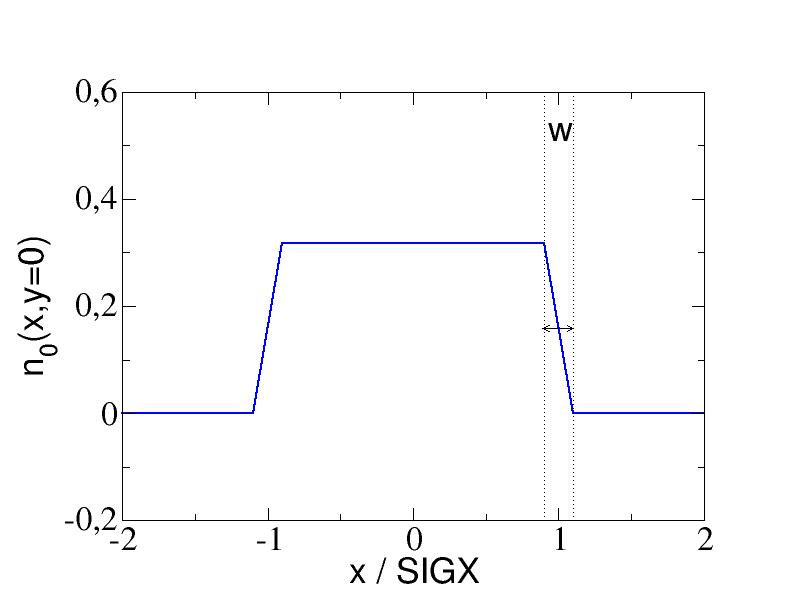
\includegraphics[width=400bp]{jpg/beambeam_n_trapez.jpg}
  \caption{Trapezoidal shape of radial density for beam-beam lens.} 
  \label{fig:beambeam-n-trapez}
\end{figure}

       \item  \texttt{BBSHAPE=3}: hollow-parabolic shape (see
       fig.\ref{fig:beambeam-n-hollowparabol}). \texttt{SIGX, SIGY} are
       the distances from the centre to the maximum of the parabolic
       density profile in horizontal and vertical directions. \\
       Only circular opposite beam is possible, \textsl{i.e.} in the
       calculations \texttt{SIGX' = SIGY' = (SIGX+SIGY)/2} is 
       used, if \texttt{SIGX} and \texttt{SIGY} have different
       values. \\
       \texttt{WIDTH} denotes the full width at half 
       maximum of the parabolic density profile in units of
       \texttt{SIGX}, or \texttt{SIGX'} and \texttt{SIGY'},
       respectively, if \texttt{SIGX} and \texttt{SIGY} are  
       not equal. Condition: \texttt{WIDTH \textless SQRT(2.0)}

\begin{figure}[h]
  \centering
  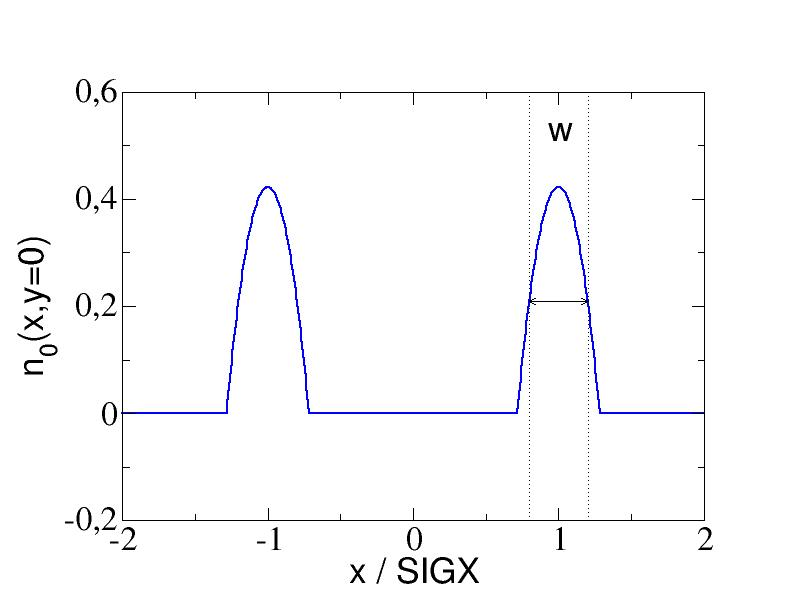
\includegraphics[width=420bp]{jpg/beambeam_n_hollowparabol.jpg}
  \caption{Hollow parabolic shape of radial density for beam-beam lens.} 
  \label{fig:beambeam-n-hollowparabol}
\end{figure}

     \end{itemize}
     
     The restriction to circular opposite beams in the cases \texttt{BBSHAPE=2,3}
     appears to be sufficient, because such beam profiles are more important 
     for the description of the interaction between the particle beam and 
     an electron beam of an electron cooler, which are usually circular. 
     
   
   \ttitem{BBDIR} A parameter to select the direction of motion of the 
     opposite beam relative to the beam being studied. It determines 
     the sign of the Lorentz force between both beams (default: -1): 
     \begin{itemize}
        \item  \texttt{BBDIR=-1}: Beams move in opposite directions as in a 
        collider. The Lorentz force enhances the beam-beam interaction. 
        \item  \texttt{BBDIR=0}: Opposite beam does not move. The Lorentz force is 
        neglected 
        \item  \texttt{BBDIR=1}: Beams move in the same direction as in an 
        electron cooler. The Lorentz force reduces the beam-beam interaction. 
     \end{itemize}
     Note:  
     \begin{itemize}  
        \item  The particles in the beam considered may have a momentum 
        deviation given by \texttt{DELTAP} defined in the
        \hyperref[sec:track]{\texttt{TRACK}} command.  
        \item  The opposite beam is assumed to have the velocity according to 
        the unperturbed energy of the particles in the beam considered. Only 
        the direction of motion can be chosen. 
        \item  In the case of motion in the opposite direction
        (\texttt{BBDIR=-1}), the time of interaction between the beams
        is given by \texttt{tau=length/(2*beta*clight)}, where
        \texttt{length} is the length of a bunch in the opposite beam.
        In the case of motion in the same direction (\texttt{BBDIR=1})
        as in an electron cooler, this time is given by
        \texttt{tau=length/(beta*c\_light)}, where \texttt{length} is
        the length of the cooler. Note that the factor 1/2 is inserted
        only for \texttt{BBDIR=-1} to calculate correct results. 
     \end{itemize}
     
\end{madlist}


A beam-beam element requires the particle
\hyperref[sec:beam]{\texttt{ENERGY}} and the particle
\hyperref[sec:beam]{\texttt{CHARGE}}, as well as the number of particles
per bunch (\hyperref[sec:beam]{\texttt{NPART}}) to be set by a
\hyperref[sec:beam]{\texttt{BEAM}} command before any 
calculation is performed. 

Example of a four-dimensional beam-beam element definition in Collider
regime: 
\madxmp{
beam,   particle = positron, npart = 1.e12, energy = 50.0; \\
bb:     beambeam, sigx = 1.e-3, sigy = 5.e-4, charge = 1.;
}


Example of a four-dimensional beam-beam element definition in an
Electron cooler:  
\madxmp{
gamma0 = 1.032;                          \= ! relativistic factor \\
beta0 = sqrt(1.0-1.0/gamm0/gamma0);      \>  \\
\> \\
i\_e = 0.2;                              \> ! electron current \\
re\_cool = 0.01;                         \> ! electron beam radius \\
l\_cool = 5.0;                           \> ! cooling length \\
\\
nelect = i\_e*l\_cool/beta0/clight/qelect; ! electron number in e-cooler \\
\\
beam, particle=antiproton, gamma=gamma0, npart=nelect;  \\
bb\_ecool: beambeam, sigx=re\_cool, sigy=re\_cool, bbshape=2, \\
\hskip 4.2cm                     width=0.01, charge=-1, bbdir=1;
}


%  Changed by: Frank Schmidt, 25-June-2003 
\section{Arbitrary Matrix Element}

\madbox{
label: MATRIX, \= TYPE=string, L=real,  \\
               \> KICK1=real,..., KICK6=real, \\
               \> RM11=real, ..., RM66=real, \\
               \> TM111=real, ..., TM666=real;
}

The \texttt{MATRIX} element allows the definition of an arbitrary transfer matrix. 
It has four real array attributes: 
\begin{madlist}
   \ttitem{L} Length of the element, which may be zero. 
   \ttitem{KICKi} Defines the kick of the element acting on the six phase
     space coordinates.  
   \ttitem{RMik} Defines the linear transfer matrix ($6\times6$ terms) of the element.  
   \ttitem{TMikl} Defines the second-order terms ($6\times6\times6$ terms) of the element. 
\end{madlist}

Data values that are not explicitly entered are taken from the identity
transformation for the \texttt{RMik} matrix elements, and taken as zero
for the \texttt{KICKi} kick factors and the \texttt{TMikl} second order
terms. 
In the \hyperref[chap:thintrack]{thin-lens tracking
module} a non-zero length for an arbitrary matrix is accepted, however
no non-zero second order terms are allowed to avoid non symplectic
tracking runs. In the latter case the tracking run is aborted.


%\section{Coordinate Transformations}
\section{Rotation around the vertical axis}
\label{sec:yrotation}

The element \texttt{YROTATION} rotates the
\hyperref[subsec:local-straight]{straight reference system} about the
vertical (\textit{y}) axis.

\madbox{
label: YROTATION, ANGLE=real;
}

\texttt{YROTATION} has no effect on the beam, but it
causes the beam to be referred to the new coordinate system  \\
\begin{equation}\begin{split}
x_2 &= x_1 \cos\theta - s_1 \sin\theta \\
s_2 &= x_1 \sin\theta + s_1 \cos\theta
\end{split}\end{equation}
%%\textit{x}$_2$=\textit{x}$_1$cos(theta)-\textit{s}$_1$sin(theta), \\
%%\textit{y}$_2$=\textit{x}$_1$sin(theta)+\textit{s}$_1$cos(theta).\\

It has one real attribute: 
\begin{madlist}
   \ttitem{ANGLE} The rotation angle $\theta$ (default: 0 rad).  
\end{madlist}

A positive angle means that the new reference system is rotated
clockwise about the local \textit{y}-axis with respect to the old system. 

\textbf{Important note:} \\
The rotation angle $\theta$ must be \emph{small}, \textsl{i.e.} it must be at
most comparable to the transverse angles of the orbit. 

Example: 
\madxmp{
KINK: YROTATION, ANGLE = 0.0001;
}

\section{Rotation around the longitudinal axis}
\label{sec:srotation}

The element \texttt{SROTATION} rotates the
\hyperref[subsec:local-straight]{straight reference system} about the
longitudinal (\textit{s}) axis. 

\madbox{
label: SROTATION, ANGLE=real;
}

\texttt{SROTATION} has no effect on the beam, but it causes the beam to be 
referred to the new coordinate system \\ 
\begin{equation}\begin{split}
x_2 &= x_1 \cos\psi - y_1 \sin\psi \\
y_2 &= x_1 \sin\psi + y_1 \cos\psi
\end{split}\end{equation}

%%\textit{x}$_2$=\textit{x}$_1$cos(psi)-\textit{y}$_1$sin(psi),\\
%%\textit{y}$_2$=\textit{x}$_1$sin(psi)+\textit{y}$_1$cos(psi).\\ 

It has one real attribute: 
\begin{madlist}
   \ttitem{ANGLE} The rotation angle $\psi$ (default: 0 rad) 
\end{madlist}

A positive angle means that the new reference system is rotated
clockwise about the \textit{s}-axis with respect to the old system.  

Example: 
\madxmp{
ROLL1: SROTATION, ANGLE=  PI/2.; \\
ROLL2: SROTATION, ANGLE= -PI/2.; \\
HBEND: SBEND, L=6.0, ANGLE=0.01; \\
VBEND: LINE=(ROLL1,HBEND,ROLL2); \\
}
The \texttt{VBEND} definition above is a way to represent a bend down in the
vertical plane, it could be defined more simply by  
\madxmp{
VBEND: SBEND, L=6.0, K0S=0.01/6;
}

\section{Coordinate translation}
\label{sec:translation}

The element \texttt{TRANSLATION} changes the
\hyperref[subsec:local-straight]{reference system} 
by applying a translation of the reference system.

\madbox{
label: TRANSLATION, \= X=real,  \= Y=real,  \= T=real, \\
                    \> PX=real, \> PY=real, \> PT=real;
}

\texttt{TRANSLATION} has no effect on the beam, but it causes the beam to be 
referred to the new coordinate system translated by the vector given. 


\section{Change of reference system}
\label{sec:changeref}

The element \texttt{CHANGEREF} changes the
\hyperref[subsec:local-straight]{reference system} 
by applying both translations and rotations.

\madbox{
label: CHANGEREF, \= PATCH\_ANG={real, real, real}, \\
                  \> PATCH\_TRANS={real, real, real};
}

\texttt{CHANGEREF} has no effect on the beam, but it causes the beam to
be referred to the new coordinate system where both translations and
rotations are applied.  

%%% END
